\documentclass{article}
\usepackage{amsmath}
\usepackage{hyperref}
\usepackage{tikz}
\usepackage{tkz-euclide}
\begin{document}

\title{Fourier Transforms of Rectangular Functions and FreeDV Filtering}
\maketitle

\section{Introduction}

Using Fourier Transforms of Rectangular Functions, this document derives expressions for generating FreeDV band pass filter coefficients at run time, and efficient implementations of the filters.

\section{Continuous Time Continuous Frequency}

Consider a rectangular function in continuous time \cite{wikipedia_rect}:
\begin{equation}
rect(t)= 
	\begin{cases}
      1, & |t| <= T/2 \\
      0, & otherwise
	\end{cases}
\end{equation}

\begin{figure}[h]
\caption{Rectangular Function in Continuous Time}
\vspace{5mm}
\label{fig:rect_time}
\centering
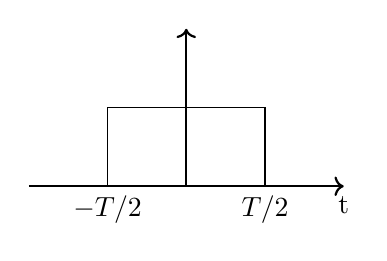
\begin{tikzpicture}
\draw[thick,->] (1,0) -- (5,0) node [below]{t};
\draw[thick,->] (3,0) -- (3,2) ;
\draw (2,0) node [below]{$-T/2$} -- (2,1) -- (4,1) -- (4,0) node [below]{$T/2$};
\end{tikzpicture}
\end{figure}

The continuous time, continuous frequency Fourier Transform is given by:
\begin{equation} \label{eq:ctcf}
\begin{split}
X(w) &= \int_{-\infty}^{\infty} rect(t)e^{-j \omega t} dt\\
     &= \int_{-T/2}^{T/2} e^{-j \omega t} dt \\
     &= \left[ \frac{1}{-j \omega} e^{-j \omega t} \right]_{-T/2}^{T/2} \\
     &= \frac{1}{-j \omega} \left[  e^{-j \omega \frac{T}{2}} - e^{j \omega \frac{T}{2}} \right] \\
     &= \frac{2 sin(\omega T/2)}{\omega} \\
     &= T sinc \left( \frac{\omega T}{2} \right) \\
\end{split}
\end{equation}
where $sinc(x) = sin(x)/x$.    

\section{Discrete Time Continuous Frequency}

Consider a rectangular function in discrete time:
\begin{equation}
rect(n)= 
	\begin{cases}
      1, & n=0,1, \ldots N-1 \\
      0, & otherwise
	\end{cases}
\end{equation}

\begin{equation} \label{eq:dtcf}
\begin{split}
                     X(w) &= \sum_{n=-\infty}^{\infty} rect(n) e^{-j \omega n} \\
                          &= \sum_{n=0}^{N-1} e^{-j \omega n} \\
                          &= e^{-j \omega 0} + e^{-j \omega 1} + ... + e^{-j \omega (N-1)} \\
       e^{-j \omega} X(w) &= e^{-j \omega} + e^{-j \omega 2} + e^{-j \omega 3} + ... + e^{-j \omega N} \\
X(w) - e^{-j \omega} X(w) &= 1 - e^{-j \omega N} \\
                     X(w) &= \frac{1 - e^{-j \omega N}}{1 - e^{-j \omega}} \\
\frac{e^{j \frac{\omega N}{2}}}{e^{j \frac{\omega}{2}}} X(w) &= \frac{e^{j \frac{\omega N}{2}}(1 - e^{-j \omega N})}{e^{j \frac{\omega}{2}}(1 - e^{-j \omega})} \\
e^{j \frac{\omega (N-1)}{2}} X(w) &= \frac{e^{j \frac{\omega N}{2}} - e^{-j \frac{\omega N}{2}}}{e^{j \frac{\omega}{2}} - e^{-j \frac{\omega}{2}}} \\
X(w) &= e^{-j \frac{\omega (N-1)}{2}} \frac{sin(\frac{\omega N}{2})}{sin(\frac{\omega}{2})}
\end{split}
\end{equation}
This can be interpreted as a complex term representing a linear phase shift (delay), multiplied by a real valued magnitude term.  For small $\omega$, the denominator term $sin(a) \approx a$, which results in a magnitude spectrum similar to the continuous time Fourier Transform (Equation \ref{eq:ctcf}).

Equation \ref{eq:dtcf} can also be derived using the closed form expression for the sum of a geometric series:
\begin{equation} \label{eq_geosum}
\sum_{k=0}^{K-1} ar^k = a \left( \frac{1-r^n}{1-r} \right)
\end{equation}

\section {Low Pass Filter Design}

Consider a continuous frequency rectangular function:
\begin{equation} \label{eq:h_omega}
H(\omega)= 
	\begin{cases}
      1, & |\omega| <= B/2 \\
      0, & otherwise
	\end{cases}
\end{equation}

\begin{figure}[h]
\caption{Rectangular Function in Continuous Frequency}
\vspace{5mm}
\label{fig:rect_freq}
\centering
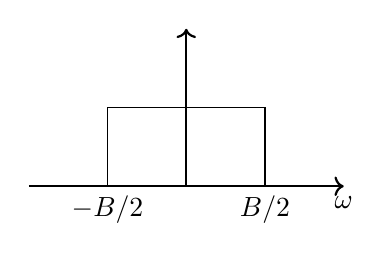
\begin{tikzpicture}
\draw[thick,->] (1,0) -- (5,0) node [below]{$\omega$};
\draw[thick,->] (3,0) -- (3,2) ;
\draw (2,0) node [below]{$-B/2$} -- (2,1) -- (4,1) -- (4,0) node [below]{$B/2$};
\end{tikzpicture}
\end{figure}

$H(\omega)$ can be considered an ideal low pass filter for real input signals, with bandwidth $B/2$ radians. The discrete time, continuous frequency inverse Fourier Transform is given by:
\begin{equation} \label{eq:dtcf_1}
\begin{split}
h(n) &= \frac{1}{2 \pi} \int_{-\pi}^{+\pi} H(\omega )e^{j \omega n} d\omega \\
     &= \frac{1}{2 \pi} \int_{-B/2}^{+B/2} e^{j \omega n} d\omega \\
     &= \frac{1}{2 \pi jn} \left[ e^{j \omega n} \right]_{-B/2}^{+B/2} \\
     &= \frac{1}{2 \pi jn} \left[ e^{j n B/2} - e^{-j n B/2} \right] \\
     &= \frac{sin \left( \frac{nB}{2} \right) }{\pi n} \\
     &= \left( \frac{\frac{B}{2 \pi}}{\frac{B}{2 \pi}} \right ) \frac{sin \left( \frac{nB}{2} \right) }{\pi n} \\
     &= \frac{B}{2 \pi} sinc \left( \frac{nB}{2} \right) \\
\end{split}
\end{equation}
Where $sinc(x) = sin(x)/x$.  Note the normalised sinc function $sinc(x) = sin(\pi x)/(\pi x)$ is common in DSP software such as GNU Octave.

The infinite length even sequence $h(n)$ can be considered the time domain impulse response of an ideal low pass filter with cut off frequency $B/2$ radians. In practice filters are limited to $N_{tap}$ taps by applying a tapered window.  This results in non-ideal frequency response, rather than an ideal rectangular (brick wall) filter. A suitable length $N_{tap}$ set of Hanning windowed filter coefficients can be found by:
\begin{equation}
\begin{split}
c(i) &= h \left( i-\frac{N_{tap}-1}{2} \right) w(i) \quad i=0 \ldots N_{tap}-1 \\
w(i) &= 0.5 - 0.5cos \left( \frac{2 \pi}{N_{tap}-1} \right)
\end{split}
\end{equation}
This expression can be used when $N_{tap}$ is odd or even.

One use case is filtering an OFDM modem signal which has significant side lobe energy at frequencies outside of the carriers. In this use case, we wish to have the filter -1dB point at a frequency just outside the carriers, in order to minimise distortion to the PSK constellation.  For a given $N_{tap}$, the smallest $B/2$ can be found by experiment that produces acceptable distortion of the scatter diagram.

To filter an input signal $X(n)$ we convolve it with the impulse response $h(n)$:
\begin{equation} \label{eq:filter_conv}
y(n) = \sum_{k=0}^{N_{tap}-1} h(k) x(n-k)
\end{equation}

\section{Complex Band Pass Filter}

Equation \ref{eq:h_omega} can be considered a low pass filter of bandwidth $B/2$ radians for real valued signals, or a bandpass filter with centre frequency 0 radians and bandwidth $B$ radians for analytic (single sided complex valued) signals. This suggests the low pass prototype filter can be shifted in frequency to construct a bandpass filter for analytic signals. 

Given the low pass prototype coefficients $h(n)$, we wish to design a band pass filter:
\begin{equation} \label{eq:h_omega_bp}
  H_{\alpha}(\omega)= 
	\begin{cases}
      1, & \alpha - B/2 <= \omega <= \alpha + B/2 \\
      0, & otherwise
	\end{cases}
\end{equation}
Where $\alpha$ is the centre frequency of the bandpass filter of bandwidth $B$.  

\begin{figure}[h]
\caption{Bandpass Filter}
\vspace{5mm}
\label{fig:bandpass_freq}
\centering
\begin{tikzpicture}
\draw[thick,->] (-5,0) -- (5,0) node [below]{$\omega$};
\draw[thick,->] (0,0) -- (0,2) ;
\draw (2,0) node [below]{$\alpha-B/2$} -- (2,1) -- (4,1) -- (4,0) node [below]{$\alpha+B/2$};
\end{tikzpicture}
\end{figure}

\begin{figure}[h]
\caption{Bandpass Filter Signal Processing}
\label{fig:bandpass_proc}
\vspace{5mm}
\begin{center}
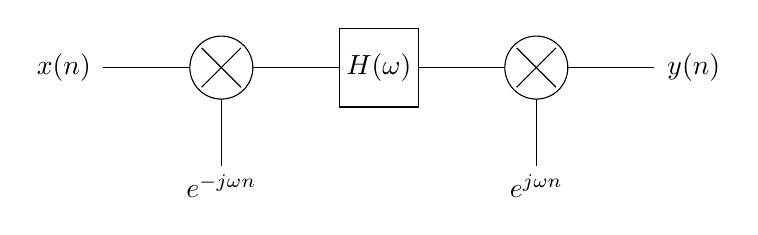
\begin{tikzpicture}
\draw (1,2) -- (2.1,2);
\draw (2.5,0.75) -- (2.5,1.6);

\draw (2.5,2) circle (0.4);
\draw (2.25,2.25) -- (2.75,1.75);
\draw (2.25,1.75) -- (2.75,2.25);

\draw (2.9,2) -- (4,2);
\draw (4,1.5) rectangle (5,2.5);
\draw (5,2) -- (6.1,2);

\draw (6.5,2) circle (0.4);
\draw (6.25,2.25) -- (6.75,1.75);
\draw (6.25,1.75) -- (6.75,2.25);
\draw (6.5,0.75) -- (6.5,1.6);

\draw (6.9,2) -- (8,2);

\node[] at (0.5,2) {$x(n)$};
\node[] at (2.5,0.5) {$e^{-j \omega n}$};
\node[] at (6.5,0.5) {$e^{j \omega n}$};
\node[] at (4.5,2) {$H(\omega)$};
\node[] at (8.5,2) {$y(n)$};
\end{tikzpicture}
\end{center}
\end{figure}

Consider the time domain sequence of operations in Figure \ref{fig:bandpass_proc}:
\begin{equation} \label{eq:bandpass_time}
y(n) = e^{j \alpha n} \sum_{k=0}^{N_{tap}-1} h(k) x(n-k) e^{-j \alpha (n-k)}
\end{equation}
Here we frequency shift the input energy in $x(n)$ centred on $\alpha$ down to 0, filter with the low pass filter $H(\omega)$, and shift the result back up to a centre frequency of $\alpha$, effectively implementing the band pass filter in Equation \ref{eq:h_omega_bp}.  Re-arranging Equation \ref{eq:bandpass_time}:
\begin{equation} \label{eq:bandpass_time2}
\begin{split}
y(n) &= e^{j \alpha n} \sum_{k=0}^{N_{tap}-1}  h(k) x(n-k) e^{-j \alpha n} e^{j \alpha k} \\
     &= \sum_{k=0}^{N_{tap}-1} h(k) e^{j \alpha k} x(n-k) \\
     &= \sum_{k=0}^{N_{tap}-1} h_{\alpha}(k) x(n-k) \\
h_{\alpha}(k) &= h(k) e^{j \alpha k}     
\end{split}
\end{equation}
Note $h_{\alpha}(k)$ is complex, and can be pre-computed from $h(n)$ at initialisation time. An alternative approach to deriving Equation \ref{eq:bandpass_time2} would be to find $h_{\alpha}(k)$ directly from the inverse FT of \eqref{eq:h_omega_bp}.

\subsection{CPU Load}

Each operation in the summation of \ref{eq:bandpass_time2} is complex so requires $4N_{tap}$ Multiply Accumulates (MACs) to compute each $y(n)$, or for a block of $N$ samples, $4N_{tap}N$ MACs.

In contrast, Equation \ref{eq:bandpass_time} has real coefficients, so for complex $x(n)$ requires $2N_{tap}$ MACs to compute each $y(n)$, plus 4 MACs each for the up and down frequency shifts. We assume $e^{-j \alpha n}$ is stored as a look up table and requires no MACs. Alternatively it can be computed using a recursion with an additional 4 MACs/sample. The up and down conversions are conjugates so only one needs to be computed, the other can then be obtained by a sign change. For a block of $N$ samples, this is a total of $(2N_{tap}+8)N$ MACs.

Table \ref{eq:bandpass_time} presents the MACs required to process a 100ms ($N=800$ samples at $Fs=8000 Hz$) block of samples.  In this example the real coefficient algorithm in Equation \ref{eq:bandpass_time} is the most efficient.

\begin{table}[h]
\centering
\begin{tabular}{l l }
 \hline
 Algorithm & MACs \\
 \hline
 Real $h(k)$ & 166,400 \\
 Complex $h_{\alpha}(k)$  & 320,000 \\ 
 \hline
\end{tabular}
\caption{Multiply Accumulates (MACs) to bandpass filter a $N=800$ block of samples using a $N_{tap}=100$ filter}
\label{table:ratek1_mean_E}
\end{table}

\section{Filter Implementation}

Consider filtering a block of $N$ samples:
\begin{equation} \label{eq:filter_block}
y(n) = \sum_{k=0}^{N_{tap}-1} h(k) x(n-k) \quad n=0,1, \ldots N-1
\end{equation}
This requires a filter memory of previous $N_{tap}-1$ samples of $x(n)$ to be maintained.  For efficient implementation we wish to avoid managing this memory during the inner MAC, for example manipulating pointers or shifting samples in a delay line. An efficient algorithm is:
\begin{enumerate}
\item At initialisation time, set up an array of $N_{tap}-1+N$ samples, initialise the first $N_{tap}-1$ samples to zero.
\item Copy the latest $N$ input samples into the last $N$ samples of the array
\item Evaluate Equation \ref{eq:filter_block} over the last $N$ samples of the array.
\item Update the filter memory by copying the last $N_{tap}-1$ samples of the array to the start of the array
\end{enumerate}
Steps 2-4 are repeated for each block of $N$ samples.

\section {Further Work}

\begin{enumerate}

\item Octave script to compare and plot fir1() to \ref{eq:dtcf_1}. Show effect of windowing on frequency response.

\item Maths for sample rate conversion, zero insertion, decimation.

\item Rather than selecting $B/2$ by trial and error, we could find an expression for the windowed FT $X_w(\omega)$, and solve for $B/2$ given $|X_w(\omega)|=10^{-1/20}$, where $\omega$ is the frequency of the desired -1dB point (e.g. just outside of the outermost OFDM carrier).  This could be evaluated for any $N_t$, trading off filter performance (and hence the OFDM signal spurious mask) for CPU load.  

\end{enumerate}

\bibliographystyle{plain}
\bibliography{rect_ft_refs}
\end{document}
